\documentclass[11pt, a4paper]{article}
\usepackage{graphicx, fullpage, hyperref, listings}
\usepackage{appendix, pdfpages, color}
\usepackage{indentfirst} %段首空两格 棒
\usepackage{chngpage} 
\usepackage{tocloft}            % This squashes the Table of Contents a bit
\usepackage{pdfpages}
\usepackage{multirow}
\usepackage{amsmath}
\usepackage{amssymb}
\usepackage{framed}
\usepackage[UTF8]{ctex}
\usepackage{array}%需要该宏包


\setlength\cftbeforesecskip{3pt}
\renewcommand{\contentsname}{\centerline{\textbf{Content}}}
\graphicspath{{images/}}

\usepackage{multicol}

\usepackage{graphicx}
\usepackage{epstopdf}
\hypersetup{CJKbookmarks,%
	bookmarksnumbered,%
	colorlinks,%
	linkcolor=black,%
	citecolor=black,%
	plainpages=false,%
	pdfstartview=FitH}

%%%%%%%代码语法高亮设置

\usepackage{color}

\definecolor{pblue}{rgb}{0.13,0.13,1}
\definecolor{pgreen}{rgb}{0,0.5,0}
\definecolor{pred}{rgb}{0.9,0,0}
\definecolor{pgrey}{rgb}{0.46,0.45,0.48}

\usepackage{listings}
\lstset{
	language=Java,
	showspaces=false,
	showtabs=false,
	%%%%%
	frame = single,
	stepnumber = 2,  
	numbersep = 4pt, 
	 numbers=left,
	%breakatwhitespace=false, 
	tabsize=2,  
	%%%%%
	breaklines=true,
	showstringspaces=false,
    breakatwhitespace=false, 
	commentstyle=\color{pgreen},
	keywordstyle=\color{pblue},
	stringstyle=\color{pred},
	basicstyle=\ttfamily,
	%moredelim=[il][\textcolor{pgrey}]{$$},
	%moredelim=[is][\textcolor{pgrey}]{\%\%}{\%\%},
}


%%%%%%%%代码语法高亮设置

\definecolor{MyLightYellow}{cmyk}{0,0.,0.2,0} 

\setlength{\parskip}{4pt}        % sets spacing between paragraphs
\interfootnotelinepenalty=500    % this prevents footnotes breaking across pages

\title{
\includegraphics[width=0.45\textwidth]{dg}
        \\AffectNet Dataset Description and Training Result on fer2013 \\ AffectNet数据集的具体说明和几种深层网络模型训练结果  }          % <<<<<<<<< change the title as appropriate
\author{Jiaming Nie}                    % <<<<<<<<< module code

\begin{document}
\begin{titlepage}
	
%\date{\today}
\maketitle
\addtocontents{toc}{\protect\thispagestyle{empty}} % because we don't want a page number on the title page
% Thanks to Huang Shanyue for suggesting this 




%\date{\today}
\thispagestyle{empty}  %去除首页页码

\end{titlepage}

%\tableofcontents
%\listoffigures

%\newpage



%\tableofcontents

%\listoffigures
%\listoftables
%\lstlistoflistings        


%\newpage

\section{AffectNet 基本信息}

AffectNet的标签共有8种表情,以及3种非表情标签(不需要),具体信息可见于表~\ref{tab:an_label}。
\begin{table}[htbp] 
	\begin{center}
		\caption{AffectNet数据集标签}
		\begin{tabular}{|l|l|l|}  \hline
		Category & 分类 & 数量 \\ \hline
		Neutral & 中立 & 80,276 \\ \hline
		Happy & 高兴 & 146,198 \\ \hline
		Sad & 悲伤 &  29,487 \\ \hline
		Surprise & 惊讶 & 16,288 \\ \hline
		Fear & 害怕 & 8,191 \\ \hline
		Disgust & 厌恶 & 5,264 \\ \hline
		Anger & 愤怒 & 28,130 \\ \hline
		Contempt & 轻蔑/蔑视 & 5,135 \\ \hline
		None &    非表情    & 35,322 \\ \hline
		Uncertain &  不确定 & 13,163 \\ \hline
		Non-Face &  非人脸(真实人脸)  &  88,895 \\ \hline
		\end{tabular}
		
		\label{tab:an_label}
	\end{center}
\end{table}	

11种分类共计45,6349个样本,所需7种表情(去除三种不明确的表情标签以及轻蔑(contempt)的表情标签)剩余样本总量为31,3834。



\section{EmotionNet 算法}

EmotionNet是一种基于人脸面部肌肉动作单位(Action Units)的数量和强度来对人脸表情进行标记的一种算法。

EmotionNet算法对特定表情的人脸图片进行特征提取并进行分类,输出表情的分类。其分类标签包括特定的表情标记(如高兴,悲伤等),也包括以面部表情的动作单位(AU,Action Units)进行分类。EmotionNet算法实现了实时处理图片,相对于人工标注提高了运算效率。

\subsection{特征空间 Feature Space}

EmotionNet对人脸图片进行特征空间的提取,并进行分类。Feature Space的提取通过对人脸部图片进行德劳内三角化处理(Delaunay triangulation),得到两点之间的距离以及形成三角形的角度,再组成 Feature Space。两点间的距离经过标准化处理(Normalization). 

德劳内三角化处理可见于下图~\ref{Fig:feature_space}. 

 \begin{figure}[htbp]
	
	\centering %使插入的图片居中显示
	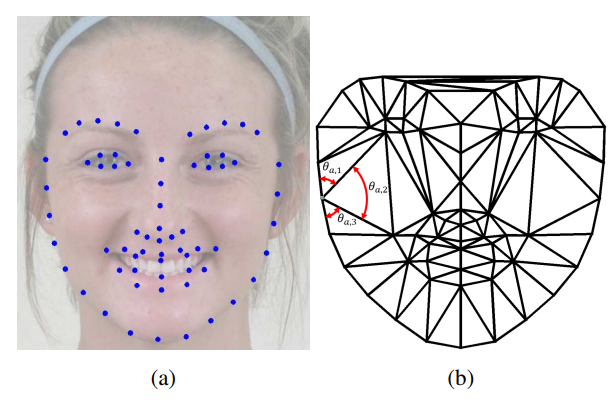
\includegraphics[width=10cm]{feature}
	
	\caption{德劳内三角化处理}
	\label{Fig:feature_space}
	%插入图片的标题,一般放在图片的下方,放在表格的上方
	
\end{figure}

图~\ref{Fig:feature_space} 所示的图片德劳内三角化处理,标记点的个数为66个,所形成的三角形个数为107个,共有321个角。

在图~\ref{Fig:feature_space} 所示的66个点中,可分为两类:

\begin{itemize}
\item[1.] 解剖学意义上的标注点(眼睛,嘴巴,嘴唇,鼻子和下巴)(共有15个)
\item[2.] 非解剖学意义标注点,这些点构成了人面部基础部分的边界,是常数,决定了人面部特征的相对位置。(原文: defining the contour of each
facial component (e.g., brows) is constant.)
\end{itemize}

\subsection{Formation of Feature Space}

对于特定的动作单位(Action Unit)${AU}_{i}$, 定义每个二维图像上的点的坐标组成的向量$s_{ij}$, 有 $s_{ij} = (s_{ij1}^{T},...,s_{ijp}^{T}{)}^{T}$。其中$s_{ijk}$ 是${AU}_{i}$上第$k$个标记点的二维坐标。

对于每个特定的${AU}_{i}$,则有132个坐标对,即$s_{ij} \in 132$。

对于每张用于训练算法的图片,距离都被标准化处理为$\tau$个像素点(pixels)。标准化处理后的$\widehat{s}_{ij} = cs_{ij}$,其中$c = \tau /{\begin{Vmatrix} l-r \end{Vmatrix}}_{2}$,$l$与$r$分别是左眼与右眼中心点的坐标。

由此可得出特征空间的表达式:

\begin{equation}
\label{eq:fv}
x_{ij} = (d_{ij12},...,d_{ijp-1p},{\theta}^{T}_{1},...,{\theta}^{T}_{p}{)}^{T}
\end{equation}

在公式~\ref{eq:fv}中,$d_{ij12} = {\begin{Vmatrix} \widehat{s}_{ija} - \widehat{s}_{ijb} \end{Vmatrix}}_{2}$ 是两点间标准化处理后的欧式距离(Euclidean Distance)。$\theta_{a} = (\theta_{a1},...,\theta_{aqa}{)}^{T}$是德劳内三角化后的角度向量。

特征向量的大小为$x_{ij} \in {\mathbb{R}}^{p(p-1)/2 + 3t}$。当$p = 66, t = 107$可得到

\begin{equation}
	x_{ij} \in {\mathbb{R}}^{2466}
\end{equation}

\subsection{Gabor Filter}

Gabor滤波器用于提取空间局部频度特征,是一种有效的纹理检测工具。

\subsubsection{Gabor Filter Equation}

\begin{equation}
g(\widehat{s}_{ijk};\lambda,\alpha,\phi,\gamma) = exp(\frac{s^{2}_{1} + \gamma_{2}s^2_{2}}{2\sigma^2})cos(2\pi \frac{s_1}{\lambda} + \phi)
\end{equation}

各种符号的标记如下:

\begin{itemize}
\item $\lambda$ - 波长
\item $\alpha$ - 方向
\item $\phi$ - 角度
\item $\gamma$ - 空间角度比例
\item $\sigma$ - 滤波器的范围
\end{itemize}

对于一个特定的$AU_{i}$, Gabor 滤波器变换后的结果为:

\begin{equation}
g_{ij} = (g^{T}_{ij1},...,g^{T}_{ijp}{)}^{T}
\end{equation}

\subsection{Final Feature Vector}

那么Feature Vector的表达式为:

\begin{equation}
	z_{ij} = (x^{T}_{ij}g^{T}_{ij}{)}^{T}
\end{equation}

\subsection{分类(Classification in Free Space)}

\subsubsection{Kernel Subclass Discriminant Analysis (KSDA)}

对于训练集的分类是基于Kernel Subclass Discriminant Analysis,KSDA 是一种基于贝叶斯网络的线性分类器,基于两条标标准对已经有的特征向量进行分类。

\begin{equation}
Q_{i1} (\phi_i,h_{i1},h_{i2}) = \frac{1}{h_{i1}h_{i2}}\sum_{c=1}^{h_{i1}}\sum_{d=h_{i1}}^{h_{i1} + h_{i2}}\frac{tr(\int_{iC}^{\phi_i}\int_{id}^{\phi_i})}{tr(\int_{iC}^{{\phi}^2_i})tr(\int_{id}^{{\phi}^2_i})}
\end{equation}

第二条标准:

\begin{equation}
Q_{i1} (\phi_i,h_{i1},h_{i2}) = \sum_{c=1}^{h_{i1}}\sum_{d=h_{i1}+1}^{h_{i1}+h_{i2}}p_{ic}p_{id}{\begin{Vmatrix} \mu_{ic}^{\phi_i} - \mu_{id}^{\phi_i} \end{Vmatrix}}^{2}_{2}
\end{equation}

\section{Fer2013 Dataset}

\subsection{基础信息}

Fer2013数据集中的图片均为$48\times 48$的灰度图片,表情的分类为7种,标记信息可见表~\ref{tab:fer2013}:

\begin{table}[htbp] 
	\begin{center}
		\caption{Fer2013}
		\begin{tabular}{|l|l|l|}  \hline
			Category & 分类 & 标记 \\ \hline
		    Angry & 愤怒 & 0 \\ \hline
		    Disgust & 厌恶 & 1 \\ \hline
		    Fear & 恐惧 & 2 \\ \hline
		     Happy & 高兴 & 3 \\ \hline 
		     Sad & 伤心 & 4 \\ \hline
		     Surprise & 惊讶 & 5 \\ \hline
		     Neutral & 中立 & 6 \\ \hline
		\end{tabular}
		
		\label{tab:fer2013}
	\end{center}
\end{table}	

\subsection{训练结果}

这里的训练结果是用一个简单的三层网络的CNN,基于keras实现。

训练中每个epoch的loss和accuracy如下(蓝线是training 红线是test):

 \begin{figure}[htbp]
	
	\centering %使插入的图片居中显示
	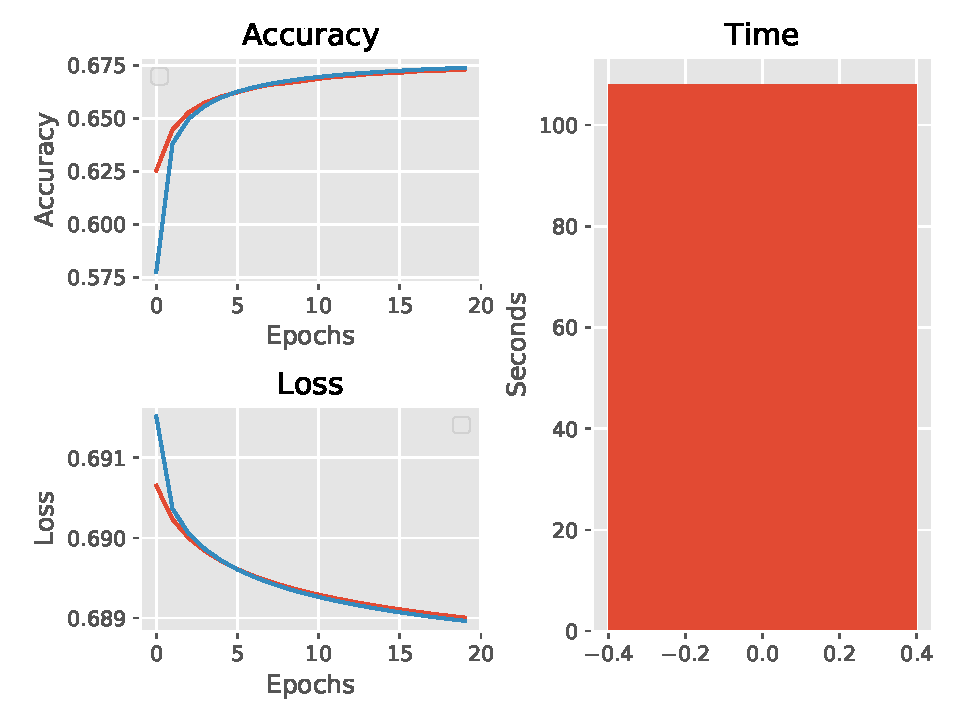
\includegraphics[width=8cm]{training}
	
	\caption{简单CNN训练结果}
	\label{Fig:training}
	%插入图片的标题,一般放在图片的下方,放在表格的上方
	
\end{figure}


\bibliographystyle{IEEEtran}  
%\bibliography{MyRefs} 
%\addcontentsline{toc}{section}{References}





%-------------------------------------------------------------------------------------------------------





\end{document}
